Una vez definido el diseño general del sistema, en este capítulo se detallan los agentes especializados que acceden a las fuentes de datos del proyecto software.

Para ello, se introduce primero la estructura de la clase base \opus{SpecializedAgent}, junto al sistema de citas integrado. Posteriormente, se detallan las herramientas y la lógica de ejecución de los cinco agentes especialistas que extienden esta base.

\section{Estructura SpecializedAgent}
El grafo común de este agente comprende tres pasos principales: la configuración del prompt inicial mediante la función \opus{prepare_prompt()}, heredada de \opus{BaseAgent} y posteriormente extendida por cada agente especialista, la ejecución de un subgrafo que implementa el patrón ReAct (véase la Sección \ref{sec:react}) y la ejecución de un agente resumidor cuando sea necesario. La Figura \ref{fig:specialized} ilustra dicho flujo de ejecución.

\begin{figure}[h]
  \centering
  \adjustbox{center=\textwidth}{\hspace{-1.2cm}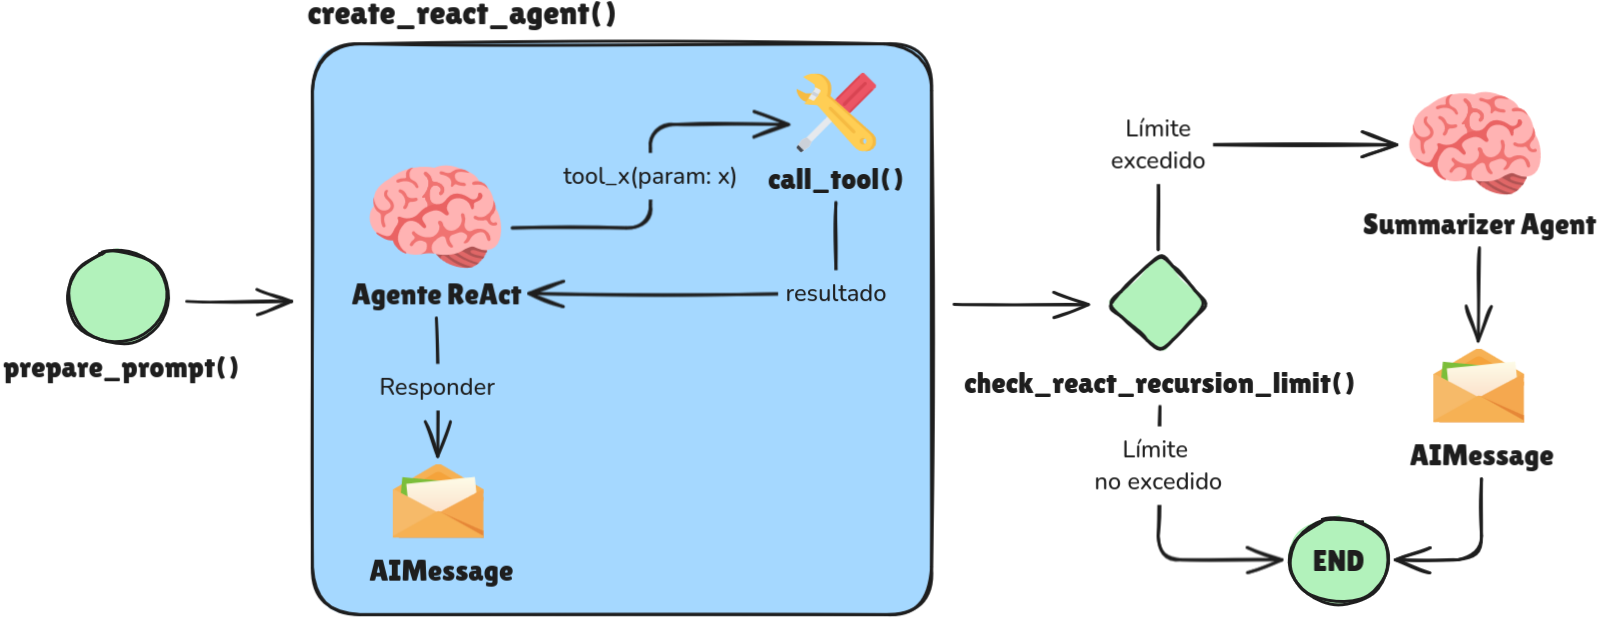
\includegraphics[width=1.2\linewidth]{figures/specialized.png}}
  \caption{Grafo de ejecución de agentes especializados}
  \label{fig:specialized}
\end{figure}

El grafo ReAct se ha implementado utilizando el agente prefabricado \opus{create_react_agent()} de LangGraph. Este agente acepta una serie de herramientas y un prompt inicial, entrando en un bucle de ejecución donde el agente invoca herramientas y observa sus resultados. El grafo finaliza cuando el mensaje del agente no contiene llamadas a herramientas, es decir, cuando incluye la respuesta final.

Se ha establecido un límite de iteraciones para el grafo ReAct, ya que se ha observado que ocasionalmente entra en un bucle excesivamente extenso al no encontrar la información requerida. Cuando se alcanza dicho límite, un agente resumidor genera una respuesta con la información disponible, observando todas las ejecuciones de las herramientas. 

El Listado \ref{lst:spec_graph} ilustra la creación del grafo para los agentes especialistas, añadiendo un nodo para cada etapa mencionada. El condicional \opus{check_react_recursion_limit} dirige la ejecución al nodo resumidor en caso de haber sobrepasado el límite de pasos en el agente ReAct.

\begin{lstlisting}[caption={\protect\opus{create_graph}: grafo de agentes especializados},label={lst:spec_graph}]
  def create_graph(self) -> CompiledGraph:
      # Crear grafo ReAct
      agent_tools = self.get_agent_tools()
      self.react_graph = create_react_agent(
          model=self.model,
          tools=agent_tools,
          checkpointer=self.checkpointer
      )

      # Crear grafo del SpecializedAgent
      graph_builder = StateGraph(SpecializedAgentState)

      # Añadir nodos 
      graph_builder.add_node("prepare", self.prepare_prompt)
      graph_builder.add_node("react", self.call_langgraph_react_graph)
      graph_builder.add_node("response_summarizer", self.generate_summarized_response)

      # Establecer flujo entre nodos: prepare -> react -> condicional -> summarizer 
      graph_builder.set_entry_point("prepare")
      graph_builder.add_edge("prepare", "react")
      graph_builder.add_conditional_edges("react", self.check_react_recursion_limit)

      return graph_builder.compile()
\end{lstlisting}

Para acceder al estado de ejecución del agente ReAct tras finalizar abruptamente por el límite de mensajes, se utiliza el sistema de autoguardado de LangGraph. En la inicialización del agente se crea un objeto \opus{AsyncPostgresSaver}, vinculado a la base de datos PostgreSQL\footnote{PostgreSQL: \url{https://www.postgresql.org/}} mediante un pool de conexión asíncrono \ref{anexo:pool} y al contexto de cierre asíncrono \opus{global_exit_stack}. De este modo, todos los estados de ejecución se almacenan en una colección de PostgreSQL y son accesibles mediante su identificador. 

\todo[inline]{Ese último párrafo creo que queda un poco denso. ¿Debería sustituirlo por este otro que omite conceptos pero es más simple?:}

Para acceder al estado de ejecución del agente ReAct tras finalizar abruptamente por el límite de mensajes, se utiliza el sistema de autoguardado de LangGraph. Mediante la clase \opus{AsyncPostgresSaver}, todos los estados de ejecución se almacenan en una colección de PostgreSQL y son accesibles mediante su identificador. 

\subsection{Gestión de herramientas}
Algunas herramientas proporcionadas por los servidores MCP resultan innecesarias o contraproducentes para determinados agentes. Para evitar incluir contenido innecesario en los prompts, se debe indicar al instanciar un agente el nombre de las herramientas que se utilizarán, filtrando posteriormente las herramientas en el cliente.

Por otra parte, algunos servidores MCP no proporcionan todas las funcionalidades requeridas. Para obtener estas herramientas adicionales, la función \opus{add_additional_tools()} incorpora, cuando es necesario, herramientas complementarias específicas para cada agente.

\subsection{Sistema de citas}
\label{sec:citas}
Para que el usuario final obtenga las fuentes de información utilizadas en la respuesta a su consulta, los agentes especializados deben referenciar los documentos consultados. Un sistema sencillo podría solicitar en el prompt que el agente indique la ruta o nombre del archivo, pero sería propenso a errores debido a que las direcciones URL de cada fuente de datos siguen patrones diferenciados. Para garantizar que los documentos citados siempre existan y contengan una dirección válida, se ha implementado el sistema ilustrado en la Figura \ref{fig:citations}.

\begin{figure}[h]
  \centering
  \adjustbox{center=\textwidth}{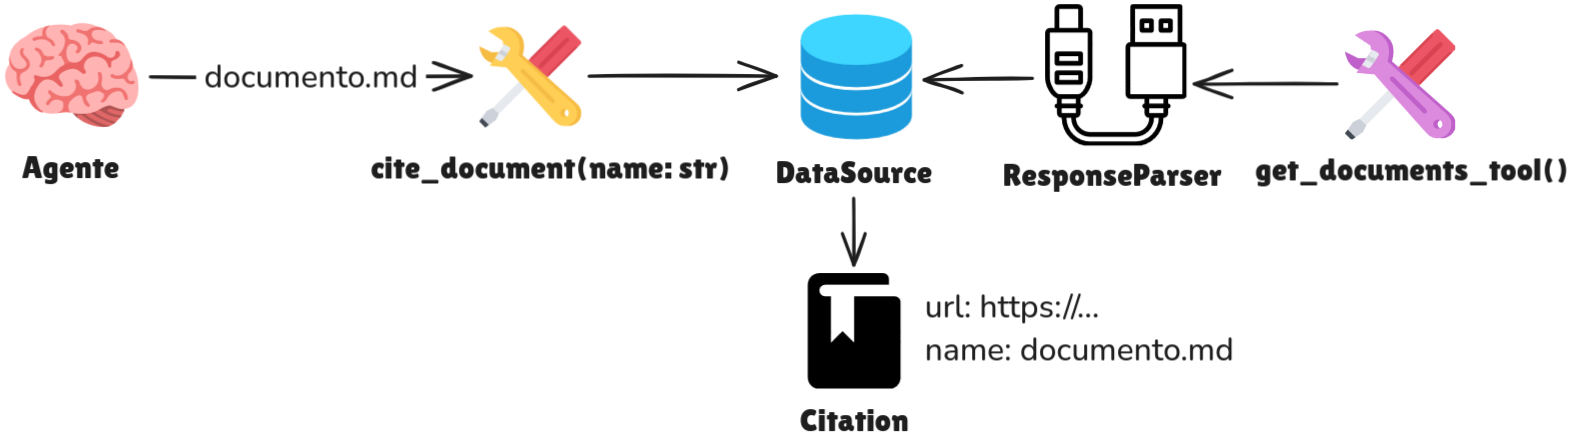
\includegraphics[width=1.1\linewidth]{figures/citations.png}}
  \caption{Diagrama de funcionamiento del sistema de citas}
  \label{fig:citations}
\end{figure}
El sistema proporciona a cada agente una herramienta para citar documentos dinámicamente construida según las fuentes a las que tiene acceso. Se implementa mediante la clase \opus{DataSource} (Listado \ref{lst:data_src}), que se inicializa utilizando herramientas específicas del servidor MCP para listar todos los documentos citables, como \opus{confluence_search()} para la fuente de datos de Confluence. Durante esta inicialización, un \opus{ResponseParser} personalizado adapta la salida de estas herramientas para extraer y catalogar los documentos en el \opus{DataSource}.

Cada \opus{DataSource} almacena la información necesaria para crear las rutas de los documentos, ensamblando automáticamente la URL completa cuando un agente necesita citar alguno de ellos. Por ejemplo, en el caso de Confluence, cada documento tiene asociado un prefijo constituido por un tipo de documento y un ID numérico en su estructura URL (\opus{url_base/tipo/id/nombre}). El \opus{DataSource} combina estos elementos para construir el enlace completo.

\begin{lstlisting}[caption={\protect\opus{DataSource}: clase destinada a almacenar los documentos citables para una fuente de datos}, label={lst:data_src}]
class DataSource(ABC):
    url: str
    # Nombre de herramienta para obtener la lista de documentos disponibles
    get_documents_tool_name: str | List[str]
    # Nombre documento -> prefijo url: {"doc_confluence.md": "page/id_9238"} 
    available_documents: dict[str, str]
    # Identificador de la fuente de datos
    docs_id: str
    parser: ResponseParser
\end{lstlisting}

Por lo tanto, el agente dispondrá de una herramienta donde bastará con indicar el nombre del documento a citar, pudiendo referenciar también la propia fuente de datos mediante el nombre especificado en la descripción de la herramienta. Las citas se propagarán mediante objetos estructurados por toda la arquitectura de agentes para imprimir finalmente las citas empleadas, como se explica en la Sección \colorbox{yellow}{\ref{}}.

\section{Agentes implementados}
En esta sección se detallan los cinco agentes desarrollados que extienden las funcionalidades descritas en la sección anterior.

\subsection{Agente código}
El flujo de este agente comprende el siguiente proceso: mediante \opus{prepare_prompt()} se incluye en el prompt del sistema el árbol de directorios del repositorio obtenido con la herramienta \opus{get_repository_tree_tool()} y fragmentos de código, denominados \textit{chunks}, relevantes para la consulta actual obtenidos mediante la herramienta \opus{get_code_repository_rag_docs_from_query_tool()}. Tras concatenar la consulta al agente mediante un \opus{HumanMessage}, este debe decidir si buscar chunks adicionales sobre un subdirectorio concreto indicando otra consulta, buscar archivos específicos con la herramienta \opus{get_file_from_repository_tool()} indicando su ruta relativa, o responder directamente a la consulta.

Los chunks devueltos por dicha herramienta contienen tanto el código como la ruta relativa del archivo donde se declaran, permitiendo buscar en dicho archivo si fuese necesario. Adicionalmente, al extraer un chunk, se incluyen chunks referenciados o que referencian ese fragmento. Se define que un chunk referencia a otro cuando llama a una función o instancia una clase definida en el otro chunk. 

\subsubsection{Herramientas de acceso a código}
\label{sec:herramientas_codigo}
Para implementar las herramientas del agente, en el componente \opus{servidor_mc_bd_codigo} se han dividido los ficheros del proyecto GitLab en chunks y se han indexado en la base de datos PostgreSQL. El sistema RAG implementado utiliza la extensión PGVector\footnote{PGVector: \url{https://github.com/pgvector/pgvector}} sobre PostgreSQL, que permite integrar vectores embeddings en tablas SQL convencionales, facilitando operaciones de búsqueda semántica combinadas con consultas SQL. 

Se ha definido el modelo relacional mostrado en la Figura \ref{fig:relacional}, utilizando el ORM SQLAlchemy\footnote{SQLAlchemy: \url{https://www.sqlalchemy.org/}} sobre Python. La estructura se basa en una tabla \opus{FileSystem} para cada fichero o directorio, que puede contener múltiples \opus{FileChunk} indexados en la columna \opus{embedding} de tipo \opus{Vector}. Cada \opus{FileChunk} puede referenciar o ser referenciado por otros \opus{FileChunk} mediante la relación muchos-a-muchos \opus{ChunkReference}. La tabla \opus{Ancestor} implementa un patrón de tabla de cierre para acceder eficientemente a los ficheros dentro de cualquier subdirectorio.

El Listado \ref{lst:rag_chunks} muestra cómo se obtienen los fragmentos más relevantes para una consulta específica. El proceso comienza desde una entrada del sistema de ficheros (\opus{FSEntry}), utiliza la tabla \opus{Ancestor} para filtrar todos los ficheros descendientes, realiza una operación de join con la tabla \opus{FileChunk} para obtener todos los fragmentos contenidos en dichos ficheros, y finalmente los ordena según su relevancia semántica respecto a la consulta del usuario.

\begin{lstlisting}[caption={Obtener chunks relevantes para una consulta dentro de un subdirectorio específico}, label={lst:rag_chunks}]
  # Filtrar primero los descendientes con la closure table
  descendant_ids = select(Ancestor.descendant_id).where(
      Ancestor.ancestor_id == fs_entry.id
  ).scalar_subquery()

  # Buscar los chunks por orden de similitud haciendo un join con la tabla de fsentry
  consulta = select(FileChunk, FileChunk.embedding.cosine_distance(query_embedding).label('distance'))\
      .join(FSEntry, FSEntry.id == FileChunk.file_id)\
      .where(FileChunk.file_id.in_(descendant_ids))\
      .order_by('distance')\
      .limit(max_results)
  results = self.db_session.execute(consulta).all()
\end{lstlisting}


\begin{figure}[h]
  \centering
  \adjustbox{center=\textwidth}{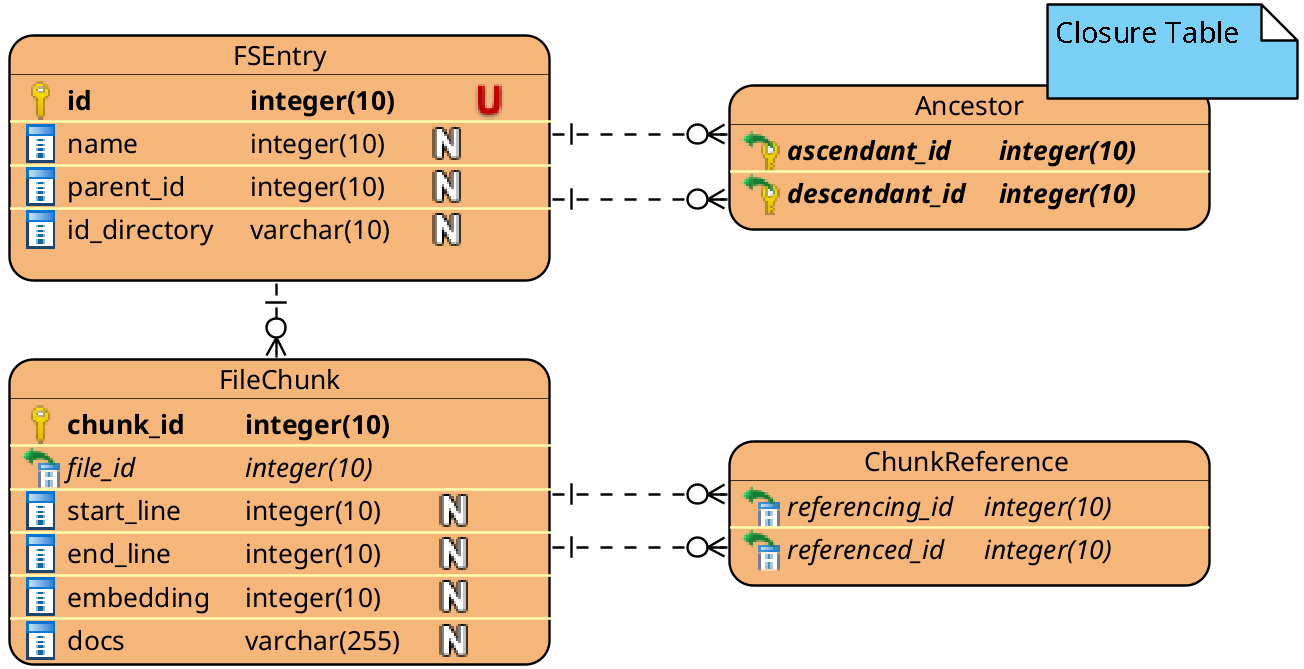
\includegraphics[width=0.95\linewidth]{figures/db.png}}
  \caption{Diagrama relacional de la base de datos con el código fuente del proyecto software}
  \label{fig:relacional}
\end{figure}

\paragraph{Procedimiento de chunking}
Para dividir los ficheros en \textit{chunks}, se han considerado las definiciones del código fuente (clases y funciones), utilizando la librería grep-ast\footnote{grep-ast: \url{https://github.com/Aider-AI/grep-ast}} para identificar definiciones y referencias en cada archivo.

La segmentación emplea un patrón State (Figura \ref{fig:state_pattern}) que recorre secuencialmente el fichero añadiendo definiciones al chunk actual hasta alcanzar su capacidad máxima. Si la siguiente definición no cabe y el chunk contiene alguna definición, se guarda el chunk actual y se inicia uno nuevo. Si el chunk está vacío pero la siguiente definición es demasiado grande, se divide: para funciones mediante segmentación equitativa, y para clases mediante subdivisión por funciones internas.

\begin{figure}[h]
\centering
\adjustbox{center=\textwidth}{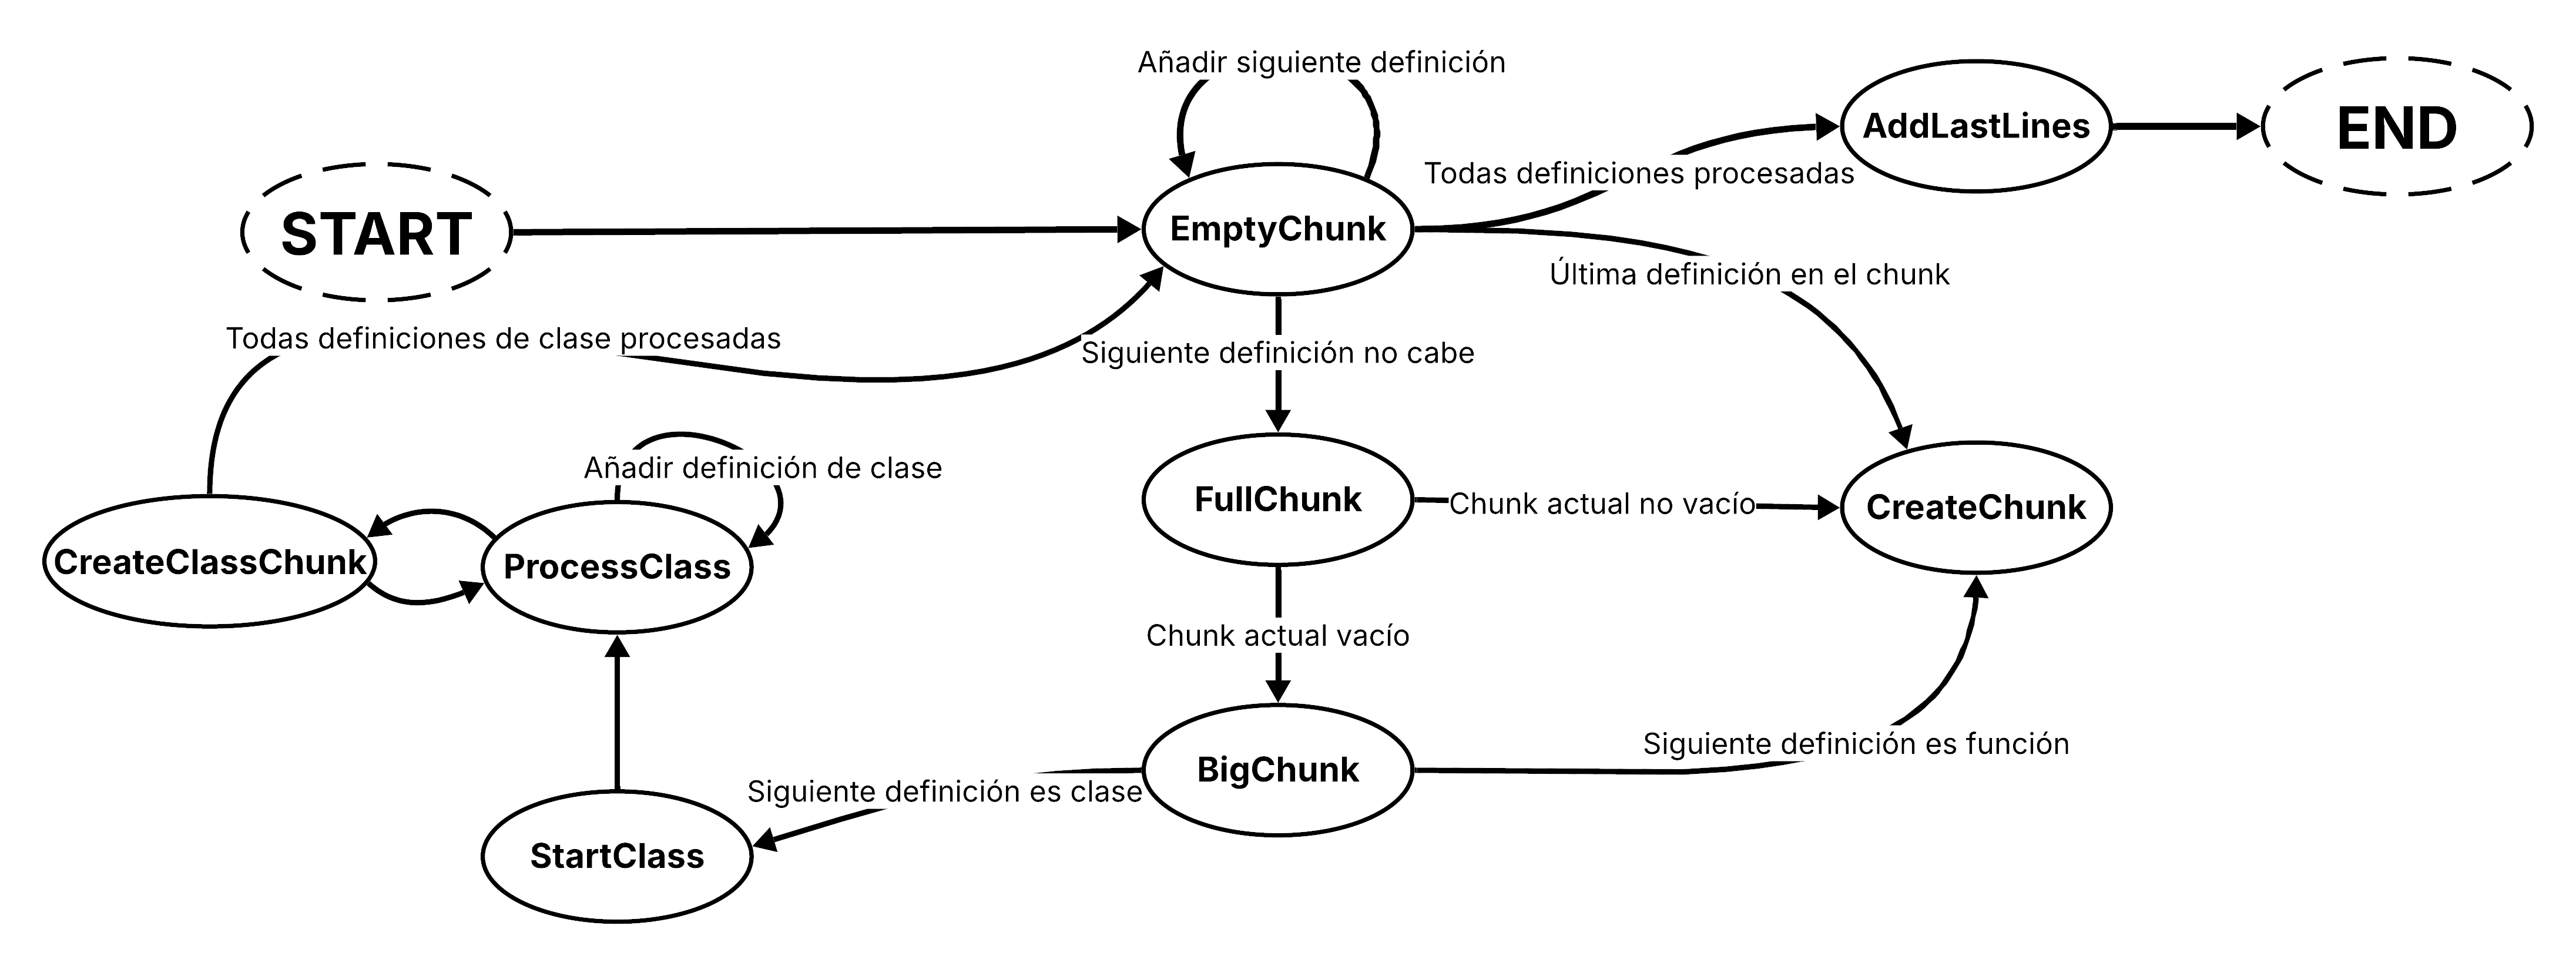
\includegraphics[width=1.35\linewidth]{figures/chunks.png}}
\caption{Algoritmo de chunking considerando definiciones de funciones y clases en el código fuente}
\label{fig:state_pattern}
\end{figure}
El proceso de chunking se implementa mediante una función recursiva que, partiendo del directorio raíz, procesa cada elemento ignorando directorios y archivos específicos. Para cada fichero, obtiene definiciones y referencias mediante grep-ast, aplica el patrón State para la división, y registra en un diccionario las definiciones declaradas con su correspondiente identificador de chunk. Finalmente, un algoritmo relaciona las referencias con sus definiciones correspondientes en el modelo relacional.

La fiabilidad del procedimiento se ha verificado mediante nueve tests unitarios de caja negra con pytest\footnote{pytest: \url{https://docs.pytest.org/en/stable/}}, ejecutados automáticamente en cada push a las ramas develop o master mediante un flujo de integración continua configurado en el archivo \opus{.github/workflows/build.yml} e integrado con SonarCloud\footnote{SonarCloud: \url{https://www.sonarsource.com/products/sonarcloud/}}.
\paragraph{Procedimiento de indexación}
Para indexar cada chunk, se ha utilizado una plantilla que considera: el código del chunk, el fichero completo, el árbol del repositorio y la documentación API generada por RepoAgent (cuya ejecución se ilustra en el Listado \ref{lst:repoagent}). Este enfoque, en lugar de indexar únicamente el código fuente, permite que las consultas posteriores encuentren fragmentos de código semánticamente relevantes al compararse con estos embeddings contextualizados.

Para ejecutar el proceso de indexación de forma estructurada y asíncrona, se ha implementado un algoritmo basado en el patrón Pipeline\footnote{Patrón Pipeline: \url{https://medium.com/@bonnotguillaume/software-architecture-the-pipeline-design-pattern-from-zero-to-hero-b5c43d8a4e60}} que desacopla la iteración de las operaciones mediante tres niveles de ejecución:
\begin{itemize}
\item\textbf{PipelinePipelineStage:} Procesos iniciales a nivel de repositorio, incluyendo la generación del árbol de directorios mediante treelib\footnote{treelib: \url{https://pypi.org/project/treelib/}} y la creación de documentación API con RepoAgent.
\item\textbf{FilePipelineStage:} Estructuración del procesamiento a nivel de fichero, permitiendo un seguimiento organizado.
\item\textbf{ChunkPipelineStage:} Operaciones para cada chunk, abarcando la creación de documentación y su posterior indexación vectorial.
\end{itemize}
La ejecución sigue un flujo jerárquico donde primero se completan las operaciones a nivel de repositorio, seguidas por el procesamiento asíncrono de ficheros y finalmente la ejecución asíncrona de operaciones a nivel de chunk, manteniendo un orden secuencial dentro de cada nivel.

\begin{lstlisting}[caption={\protect\opus{generate_extra_docs}: Ejecución de agente RepoAgent para crear la documentación API}, label={lst:repoagent}]
  def generate_extra_docs(files_to_ignore: List[str], repo_path: str, extra_docs_path: str):
      try:
          files_to_ignore_str = ",".join(files_to_ignore)
          command = f"repoagent run --model gpt-4o-mini --target-repo-path {repo_path} --markdown-docs-path {extra_docs_path} --ignore-list {files_to_ignore_str}"
          exit_code = execute_and_stream_command(command)
      ...
\end{lstlisting}

\subsection{Agente Google Drive}
La función de este agente consiste en buscar y analizar las maquetas HTML almacenadas en Google Drive. Mediante la herramienta \opus{gdrive_list_files()}, la función \opus{prepare_prompt()} proporciona al agente información sobre todos los documentos disponibles. Posteriormente, el agente determina si debe buscar fragmentos relevantes en los documentos utilizando la herramienta \opus{gdrive_search()}, o acceder a documentos completos mediante la herramienta \opus{gdrive_read_file()}.

\subsection{Agente Sistema de Ficheros}
\label{sec:agente_filesystem}
Este agente responde a consultas utilizando la documentación oficial como fuente de datos. La función \opus{prepare_prompt()} proporciona la lista de documentos disponibles a través de la herramienta \opus{directory_tree()} en el prompt inicial, pudiendo acceder a archivos específicos con \opus{read_file()} o \opus{read_multiple_files()}, o realizar búsquedas de pasajes relevantes a través de \opus{rag_search_documentation()}.

Esta última herramienta se ha implementado utilizando la clase PGVector de LangChain. A diferencia de la implementación nativa de PGVector utilizada en el agente de código, esta versión ofrece una abstracción más sencilla para búsquedas RAG, pero sacrifica la capacidad de combinar operaciones de búsqueda semántica con consultas SQL avanzadas.

Como muestra el Listado \ref{lst:pgvector_store}, se crean colecciones mediante instancias de PGVector donde una columna se vectoriza para búsqueda semántica y las demás actúan como metadatos filtrables. Entre estos metadatos se incluye la ruta del archivo indexado, lo que permite al agente identificar el origen de cada fragmento y decidir si necesita extraer el documento completo.

\begin{lstlisting}[caption={\protect\opus{PGVector}: uso de clase para indexar o buscar documentos}, label={lst:pgvector_store}]
  # Instanciar la clase en su versión asíncrona 
  vector_store = PGVector(
      embeddings=self.embeddings,
      collection_name=prefixed_name,
      connection=self.engine,
      use_jsonb=True,
      async_mode=True
  )

  # Añadir documentos (clase LangChain con texto y metadatos) al store
  await self.vector_store.aadd_documents(docs)

  # Buscar documentos similares mediante una operación vectorial
  results = await self.vector_store.asimilarity_search(query, k=top_k)
\end{lstlisting}

\subsection{Agente Confluence}
Para este agente se han implementado dos versiones alternativas: una estándar y otra con un enfoque en el cacheo del prompt.

El \textit{prompt caching} almacena la representación interna del LLM para secuencias de texto iniciales repetidas, evitando cálculos redundantes en consultas posteriores. APIs como OpenAI ofrecen descuentos significativos cuando se cachea gran parte de la entrada. La Figura \ref{fig:caching} compara ambos enfoques, donde las secciones resaltadas en rojo representan fragmentos del prompt inicial que se repiten entre diferentes llamadas y son cacheados. En ambos casos el cacheo finaliza al incorporar la consulta específica del usuario, dado que esta varía en cada interacción. Sin embargo, la segunda implementación logra cachear un volumen de texto considerablemente mayor.
\paragraph{Implementación estándar}
En esta implementación estándar, \opus{prepare_prompt()} utiliza \opus{confluence_search()} para identificar los documentos disponibles en la documentación del estilo visual, permitiendo al agente acceder posteriormente a documentos específicos mediante \opus{confluence_get_page()}.
\paragraph{Enfocado en el cacheo del prompt}
Esta versión incorpora toda la documentación directamente en el contexto de entrada, permitiendo al agente responder mediante referencias a los documentos pertinentes. Esta estrategia resulta viable únicamente cuando los documentos completos pueden incluirse dentro de la ventana de contexto del modelo.

\begin{figure}[h]
  \centering
  \adjustbox{center=\textwidth}{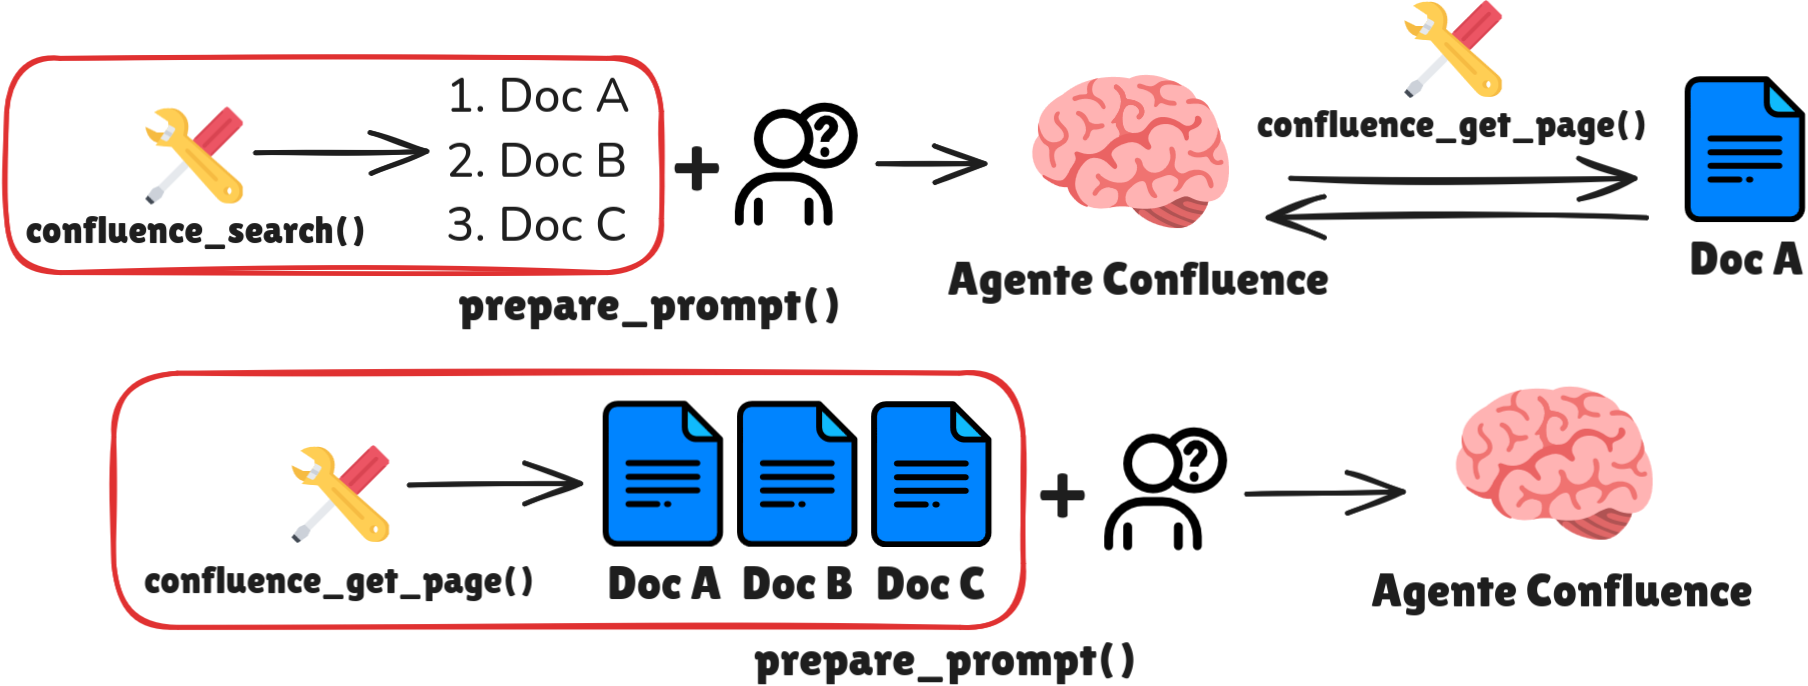
\includegraphics[width=0.85\linewidth]{figures/confluences.png}}
  \caption{Comparación de agente Confluence estándar y enfocado en el cacheo del prompt}
  \label{fig:caching}
\end{figure}

\subsection{Agente GitLab}
\label{sec:agente_gitlab}
El agente recibe inicialmente mediante \opus{prepare_prompt()} estadísticas del repositorio obtenidas a través de la herramienta \opus{get_gitlab_project_statistics()}, incluyendo datos sobre contribuciones, usuarios e incidencias. Posteriormente, puede emplear las siguientes herramientas:
\begin{itemize}
  \item\opus{get_gitlab_project_commits(user_name, since, until, result_limit):} Recupera contribuciones (\textit{commits}) con opciones de filtrado por usuario, fechas o cantidad.
\item\opus{get_gitlab_project_members():} Obtiene información sobre usuarios contribuyentes. Es de destacar que para filtrar contribuciones por usuario, el agente debe invocar primero esta herramienta para obtener los nombres de usuario en GitLab.
\item\opus{get_gitlab_branches():} Proporciona información sobre las ramas git del proyecto.
\item\opus{get_gitlab_issues():} Recupera las incidencias (\textit{issues}) registradas en el proyecto.
\end{itemize}
Cabe destacar que, en lugar de citar documentos, este agente tiene la capacidad de citar contribuciones o incidencias del repositorio.

La implementación ha requerido el desarrollo de herramientas específicas mediante la API de GitLab utilizando la librería \opus{requests}\footnote{requests: \url{https://pypi.org/project/requests/}}. Como se detalla en el Listado \ref{lst:gitlab_api}, las herramientas se crean llamando a la API con las credenciales y la URL correspondiente.

\begin{lstlisting}[caption={Ejemplo de herramienta para agente GitLab directamente desde la API},label={lst:gitlab_api}]
  # La herramienta llama a una función que gestiona la paginación en varias requests 
  @tool
  def get_gitlab_project_members():
      return execute_gitlab_api_request_with_pagination("members")
  ...

  def execute_gitlab_api_request(url: str, params: Dict[str, Any] = None) -> Response:
    gitlab_token = os.getenv('GITLAB_PERSONAL_ACCESS_TOKEN')
    request_url = f"{GITLAB_API_URL}/projects/{GITLAB_PROJECT_URL}/{url}"
    headers = { "PRIVATE-TOKEN": gitlab_token }

    return requests.get(request_url, headers=headers, params=params)
\end{lstlisting}



















